\section{Native unresolved observations: a frozen 100-event pilot}
\label{sec:real-observations}

\subsection{A separate observation contract and its identifiable quantities}

The resolved-pair experiments above are not the observation model for an
unresolved survey light curve. Release candidate 0.2.0rc3 adds a separate,
versioned native-photometry route. An input row retains its original
time, apparent magnitude, uncertainty, instrument/filter, source file hash
and source-line identity. Catalog coordinates, aliases, calibration notes
and documented warnings remain provenance. No image positions, primary
flux ratios, interimage delays, distances or covariance are manufactured
from those rows.

For a rectilinear point-source point-lens (PSPL) event
\cite{Paczynski1986}, the dimensionless source--lens separation and
unresolved magnification are
\begin{equation}
 u(t)^2=u_0^2+\left(\frac{t-t_0}{t_E}\right)^2,\qquad
 A(u)=\frac{u^2+2}{u\sqrt{u^2+4}}.
 \label{eq:native-pspl}
\end{equation}
For instrument $j$, $F_j=F_{s,j}A+F_{b,j}$. Writing the baseline
magnitude as $m_{b,j}$ and the baseline source fraction as
$f_j=F_{s,j}/(F_{s,j}+F_{b,j})$ gives the native-magnitude prediction
\begin{equation}
 m_j(t)=m_{b,j}-2.5\log_{10}\!\left[1+f_j(A(u(t))-1)\right],\qquad
 \chi^2=\sum_i\frac{[m_i-m_{j(i)}(t_i)]^2}{\sigma_i^2}.
 \label{eq:native-magnitude-likelihood}
\end{equation}
This likelihood assumes independent Gaussian errors in the supplied
native magnitudes. It preserves the supplied errors; it does not infer
an unprovided cross-row covariance or establish that the independence
assumption is correct. Per-instrument baselines absorb independent
photometric zero points without treating published catalog parameters as
new measurements. The catalog solution initializes one of twelve
deterministic starts and contributes no likelihood term.

The optical model has the same BHSM Einstein/GHY interpretation as
Section~\ref{sec:bhsm-interpretation}: one effective exterior acts once.
Unresolved PSPL photometry, however, generally constrains only event
time, dimensionless impact parameter, timescale and blending combinations,
to the extent admitted by its sampling and degeneracies. In the usual
angular convention,
\begin{equation}
 \theta_E^2=\kappa M\pi_{\rm rel},\quad
 \pi_E=\pi_{\rm rel}/\theta_E,\quad
 M=\frac{\theta_E}{\kappa\pi_E},\quad
 \mu_{\rm rel}=\theta_E/t_E,\qquad
 \kappa=\frac{4G}{c^2\,\mathrm{AU}}.
 \label{eq:native-mass-identifiability}
\end{equation}
The baseline fit measures neither $\theta_E$ nor $\pi_E$
\cite{Gould2014}. A long $t_E$ can arise from mass, relative distance or
slow relative motion. Mass, lens distance, absolute lens motion,
Schwarzschild radius, and the mass-derived boundary dictionary therefore
remain unavailable for every pilot event. No core state or deformation
is inferred from ordinary PSPL agreement. The optional astrometric
centroid and geocentric-parallax primitives have analytic convention and
input-admission tests \cite{DominikSahu2000,Gould2004}; this pilot is not
an end-to-end joint astrometric mass analysis.

\subsection{Data integrity, selection and protocol freeze}

The supplied observations are the optimized OGLE-III Class A catalog and
its native light curves \cite{Wyrzykowski2015}, together with the
separate 2022 OB110462 benchmark deposit \cite{Lam2022Data}. All 109
supplied raw-file hashes verify. The pilot exactly reproduces the frozen
100-event selection: all 75 catalog events with published $t_E\geq150$
d, and 25 hash-selected controls from 2272 eligible events with
$10\leq t_E<50$ d, in a 3560-event parent catalog. These are historical
published events. Catalog selection and long-duration enrichment prevent
a completeness, black-hole abundance or population-rate inference.
Although the original standard-event selection disfavors conspicuous
parallax/exotic events, later alias/coordinate checks find four exact
members of the published 59-event parallax sample
\cite{Wyrzykowski2016}; it is incorrect to describe the cohorts as disjoint.

All 76\,344 numeric pilot rows enter the baseline and both sensitivity
fits. The loader records four documented source annotations, retains
OGLE3-ULENS-0337, and applies no clipping, thinning, averaging, duplicate
deletion, event replacement or second application of published error
corrections. Native HJD relative-day arithmetic is sufficient for this
rectilinear screen; its underlying clock scale is retained as unspecified,
rather than guessed for a precision ephemeris calculation. The downloaded
bytes are unchanged after analysis.

Protocol \texttt{BHSM-OGLE3-native-pilot-20261022-v1} was frozen at
19:50:27 UTC on 22 October 2026 before measured-light-curve fits. Its
SHA256 is
\texttt{b1e75ea7\allowbreak{}08343bad\allowbreak{}1207ac18\allowbreak{}0229058f\allowbreak{}093164e8\allowbreak{}77cea68a\allowbreak{}c13bedfc\allowbreak{}3feed498};
the ordered event-ID digest is
\texttt{0cf5dbf7\allowbreak{}14a99567\allowbreak{}ccfc8448\allowbreak{}f5356033\allowbreak{}3ed45971\allowbreak{}15a28011\allowbreak{}38ac7079\allowbreak{}26a8a4a7}.
This is an internal frozen analysis, not external preregistration.
The protocol pins the raw data, driver, likelihood and source modules;
the completed results and later literature annotations have separate
manifests. The original kernel is retained for replay. Post-pilot
astrometry docstring clarifications change no executable syntax, and
the native-photometry and observation modules remain byte-identical.
The final rc3 theory-source update to revision \texttt{705d4c7e} is a
separately recorded provenance change; the pilot retains its original
interpretation pins and unchanged PSPL objective.

\subsection{Numerical admission, uncertainty and limited validation}

The fit uses bounded trust-region least squares with an analytic
Jacobian, twelve starts, 1500 evaluations per start, a fixed seed,
linear loss and declared stopping tolerances. Search bounds are
$0.1\leq t_E\leq10^4$ d, $10^{-4}\leq u_0\leq10$,
$10^{-6}\leq f_j\leq1$, $t_0$ within the data range extended by one
observed span on each side, and each baseline within ten magnitudes of
its instrument median. These are explicit computational/model bounds,
not measured physical limits. An active bound flags nonregular local
uncertainty. A column-normalized Jacobian SVD uses relative cutoff
$10^{-7}$; unidentified directions yield unavailable public
uncertainties rather than zero-error estimates.

Every event also has a nuisance-reoptimized timescale profile. Seventeen
log-spaced values cover $[t_E/4,4t_E]$, clipped to the declared search
range, with the fitted point included. Four deterministic source-fraction
seeds reoptimize all remaining nuisance coordinates at each trial.
Adjacent admitted converged rows bracket a $\Delta\chi^2=1$ reference
crossing, refined by up to sixteen logarithmic bisections with new
nuisance fits. A failed row blocks that crossing; a finite grid endpoint
is not a physical confidence limit. Both crossings are found for 91
events; nine remain grid-interval unresolved. These are likelihood
reference levels, not calibrated coverage intervals, especially for an
inadequate model.

Two predeclared sensitivity fits are retained for all 100 events:
uniform native-error multiplication by 1.25, and a signed-blend
phenomenology with source fraction up to ten. The latter represents
possible calibration/background offsets; it is not negative physical
stellar luminosity. Neither replaces the baseline. Diagnostics retain
multistart alternatives, active bounds, local rank, constant/linear-trend
BIC comparisons, runs and lag-one residual statistics, seasonal residual
offsets, and instrument-specific residuals.

Before real-data inference, synthetic injections on two actual sampling
patterns test the new likelihood. Noiseless $t_E=200$ d and 25 d
injections recover their parameters with $\chi^2<2\times10^{-23}$;
eight independent-noise draws at each cadence test recovery and error
scaling. A weak-source injection exposes the blending--timescale profile
degeneracy. Sixteen noise trials do not establish interval coverage,
false-discovery control or black-hole recovery. They are separate from
the historical 64- and 128-draw resolved-pair calibrations above; those
receipts retain their original code versions and are not new-kernel
coverage tests. Focused F1--F3 correction verification comprises 75 passing
tests of physical reference invariance, admitted nuisance profiles and
unidentified-motion reporting; this count is not a new observational
calibration.

\subsection{All-event outcomes and bounded follow-up ranking}

The run completes all 100 events without changing the cohort. Eighty-nine
are \texttt{PHOTOMETRIC\_\allowbreak{}MODEL\_\allowbreak{}INADEQUATE}; eleven receive
\texttt{PHOTOMETRIC\_FIT} because the specified independent-error
$\chi^2$ screen does not reject them. The latter label is not full
scientific adequacy: residual structure, boundary effects and alternative
models remain separate tests. The long-duration stratum contributes
67 inadequate and eight non-rejected fits; the controls contribute 22
and three, respectively. Failed or inadequate outcomes remain in the
released all-event table and in every denominator.

The frozen archival-follow-up screen additionally requires a finite
locally identified $\sigma_{t_E}/t_E<0.3$, both profile crossings,
confirmed multistart results, no active bounds, no prescribed runs or
seasonal residual flag, $\Delta\mathrm{BIC}>10$ relative to a linear
trend, and timescale stability in both sensitivities. Ranking then sorts
lexicographically by $|\log\chi^2_\nu|$, profile fractional half-width,
decreasing timescale and event ID. These operational criteria select two
historical objects (Table~\ref{tab:pilot-followups}); they are not
black-hole probabilities or an externally validated discovery statistic.
Figure~\ref{fig:actual-followups} shows both selected light curves and
their residuals, retaining every native observation.

\begin{figure}[p]
\centering
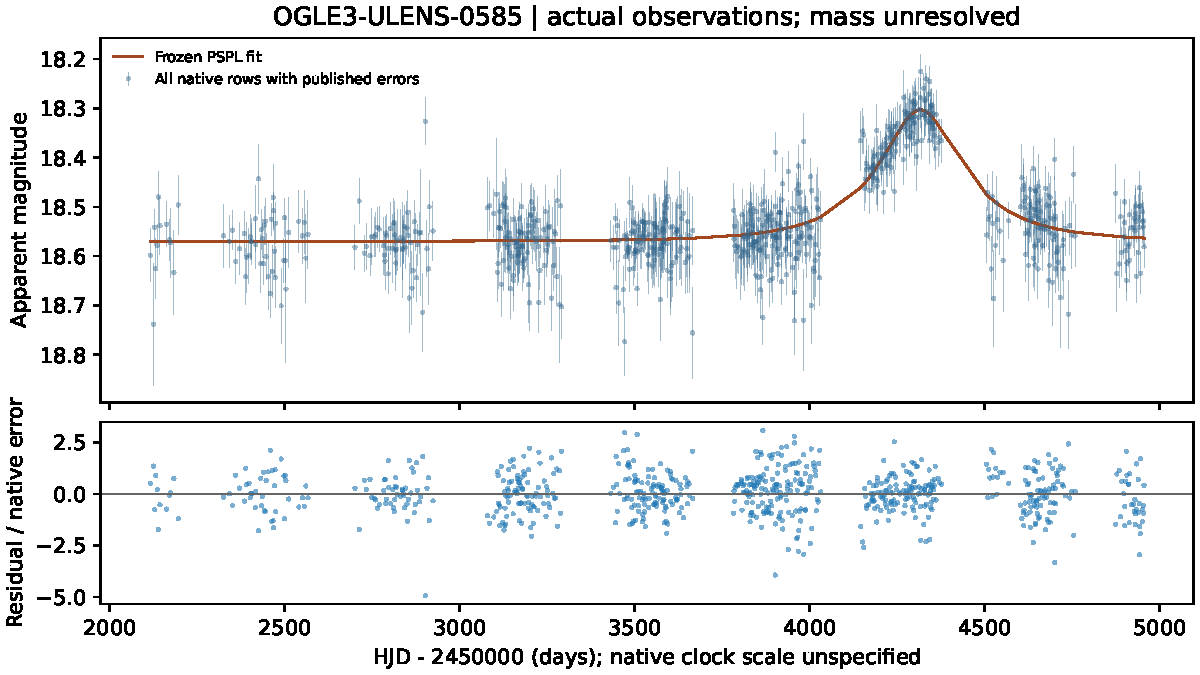
\includegraphics[width=.95\linewidth]{../figures/OGLE3-ULENS-0585_native.pdf}
\medskip
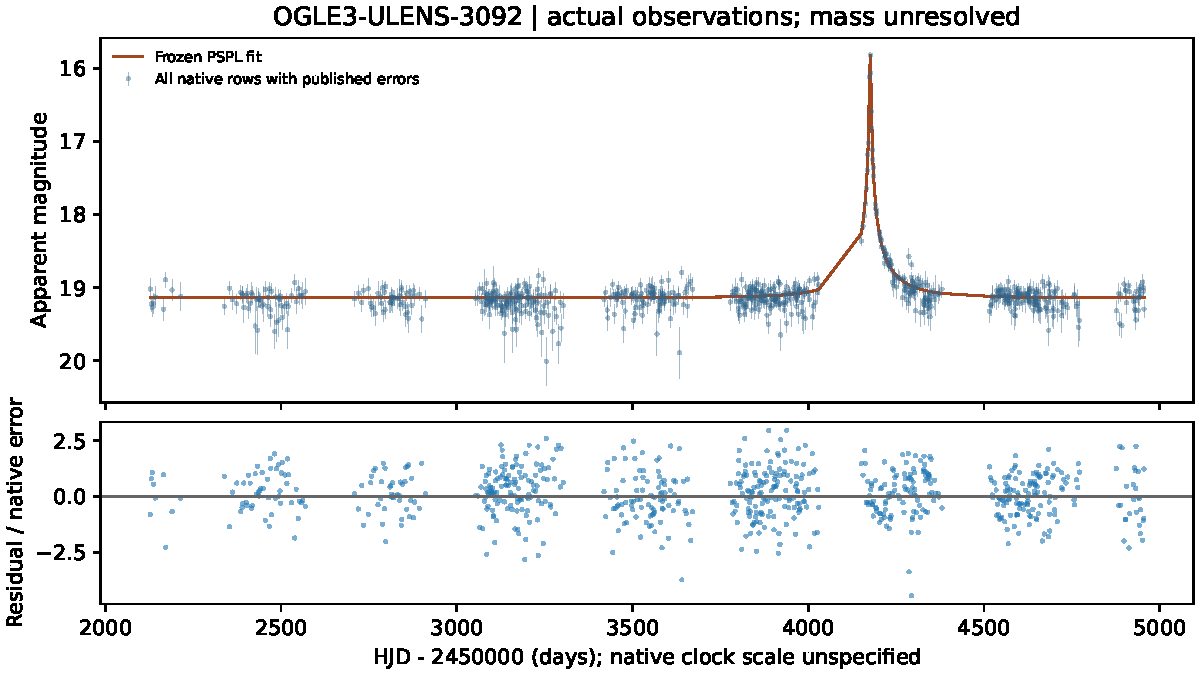
\includegraphics[width=.95\linewidth]{../figures/OGLE3-ULENS-3092_native.pdf}
\caption{Actual observations of the only two events passing the frozen
archival-follow-up screen. Curves are the saved baseline fits; bars are
the original magnitude errors, and lower panels retain all standardized
residuals. The fits identify conditional photometric combinations, not
lens mass or type. These historical events are not new discoveries.}
\label{fig:actual-followups}
\end{figure}

\begin{table}[tbp]
\centering\small
\caption{The only two events passing the frozen archival-follow-up
screen. Profile limits are nuisance-reoptimized $\Delta\chi^2=1$
reference crossings in days, without a coverage claim. Mass is
unavailable for both.}
\label{tab:pilot-followups}
\begin{tabular}{@{}lrrrr@{}}
\toprule
OGLE3-ULENS & Rows & $\chi^2/\nu$ & Fitted $t_E$ (d) & Profile (d)\\
\midrule
0585 & 734 & $748.247/729$ & 268.17 & $[202.91,344.96]$\\
3092 & 739 & $805.423/734$ & 187.73 & $[170.06,208.64]$\\
\bottomrule
\end{tabular}
\end{table}

The fitted baseline source fractions, 0.180 and 0.195, emphasize that
blending remains consequential. OGLE3-ULENS-0585 is catalog source
\texttt{BLG122.6.83113}; the supplied catalog has no EWS alias.
OGLE3-ULENS-3092 is \texttt{BLG225.6.198210}, independently associated
with OGLE-2007-BLG-057 by the official EWS coordinates (separation
0.75 arcsec). It is also MOA-2007-BLG-027, discussed by
Yock~\cite{Yock2008}; its prior high-magnification event and incomplete
peak coverage are not a new discovery. The historical EWS and optimized
catalog star identifiers belong to different reductions and are both
retained. Bounded alias/name/coordinate searches locate no specific
earlier lens-interpretation paper for 0585, but absence from this search
does not establish novelty. Neither object has measured mass here;
both are candidates for archival reanalysis and imaging feasibility,
not current alerts or credible new black-hole classifications.

The four exact prior-parallax matches in the full pilot are
0264/PAR-07, 0568/PAR-21, 2122/PAR-37 and 3404/PAR-17. In particular,
0264 was already proposed as a dark-remnant candidate in the 2016 study.
The later Gaia-informed analysis changes its conditional inference
\cite{Mroz2021}; a prior-dependent literature mass is not imported as
a mass measurement by this PSPL fit. Machine-readable literature
annotations preserve these associations alongside the unchanged frozen
results. The run yields zero mass-supported black-hole candidates and
zero new black-hole interpretations.

\subsection{The historical known-system benchmark and its stopping point}

OB110462 (OGLE-2011-BLG-0462/MOA-2011-BLG-191) is analyzed only with
the corresponding Zenodo 6607578 version 1.0.0 release
\cite{Lam2022Letter,Lam2022Supplement,Lam2022Data}, separately from the
pilot. The deposit's requested OGLE attribution is also retained
\cite{Udalski2015}. Its 15\,545 OGLE and 46\,040 MOA photometric rows
are retained. Later analyses use additional observations and revised
reductions \cite{LamLu2023,Sahu2025}; their masses and newer measurements
are not substituted for the 2022 input version.
All five specified PSPL fits converge with confirmed multistart solutions,
yet all fail the declared photometric adequacy screen and show
time-correlated/seasonal residuals (Table~\ref{tab:historical-benchmark}).
Convergence therefore cannot be presented as recovery of the published
black-hole mass. Parallax, source/lens complexity and noise calibration
require their own validated likelihoods.

\begin{table}[tbp]
\centering\small
\caption{Historical 2022-data benchmark: all entries are inadequate
photometry-only fits. The final column evaluates the native-error
$\chi^2$, including for the alternative weighting sensitivity.}
\label{tab:historical-benchmark}
\begin{tabular}{@{}lrr@{}}
\toprule
Fit/sensitivity & Fitted $t_E$ (d) & Native $\chi^2_\nu$\\
\midrule
Joint OGLE/MOA & 282.80 & 2.4515\\
OGLE only & 270.79 & 3.6754\\
MOA only & 299.06 & 2.0259\\
Equal-instrument objective & 276.47 & 2.4532\\
Signed-blend sensitivity & 282.80 & 2.4515\\
\bottomrule
\end{tabular}
\end{table}

Sixteen HST rows at eight shared visits are ingested with native column
labels, but are not used for precision joint inference. Primary-source
recovery establishes that the 2022 reduction applies a cross-filter
alignment, while a historical BAGLE reader converts private decimal-year
UTC epochs to MJD. Neither supplies the missing exact export mapping for
these deposited ASCII times. A concrete check against MAST observation
metadata finds all eight native numbers outside the matching F606W
exposure windows if naively interpreted as MJD UTC. No guessed epoch
shift or second filter offset is applied. Astrometric frame/coordinate
and covariance conventions also require verification before composition
with an ephemeris. The precision joint route consequently reports missing
verified metadata and leaves $\theta_E$, $\pi_E$ and mass unresolved.

Lam et al.'s published default weighting sums the photometric and
astrometric log likelihoods; their equal weighting divides each data-group
log likelihood by that group's count \cite{Lam2022Supplement}. The
photometry-only equal-instrument sensitivity above omits HST astrometry
and does not reproduce that published joint likelihood. This is a
version-specific benchmark of data admission and model failure, not a
replacement for either published mass analysis. The source/metadata
research, archived source hashes, raw-data provenance, all-event table,
fit diagnostics, residual plots and replay instructions are distributed
with the review material. Raw OGLE observations remain external pending
clear redistribution permission; the Zenodo deposit declares CC BY 4.0.
